% Entrega 3 (informe final). Fuente larga: entrega3/INFORME_FINAL.md.
% Estructura alineada con el enunciado (entrega3/Enunciado P3 NLP.pdf):
%   1. Correcciones finales            -> Sección II
%   2. Desarrollo del modelo final     -> Sección IV
%   3. Análisis de resultados y discusión -> Secciones V y VI
% Las cifras salen de los CSV de entrega3/resultados_publico/ (ver GUIA_ENTREGA3.md).
% Compilar desde informe/:  pdflatex entrega3.tex && pdflatex entrega3.tex
% (también compila con XeLaTeX o Tectonic).
\documentclass[10pt,twocolumn]{article}
\usepackage{iftex}
\ifPDFTeX
  \usepackage[T1]{fontenc}
  \usepackage[utf8]{inputenc}
\else
  \usepackage{fontspec}
\fi
\usepackage[spanish,es-nodecimaldot,es-tabla]{babel}
\usepackage{geometry,graphicx,booktabs,array,tabularx,caption,amsmath,amssymb,xcolor,url,hyperref}
\usepackage{newunicodechar}
\newunicodechar{Δ}{\ensuremath{\Delta}}
\newunicodechar{κ}{\ensuremath{\kappa}}
\newunicodechar{θ}{\ensuremath{\theta}}
\newunicodechar{≈}{\ensuremath{\approx}}
\newunicodechar{≥}{\ensuremath{\geq}}
\newunicodechar{≤}{\ensuremath{\leq}}
\newunicodechar{≠}{\ensuremath{\neq}}
\newunicodechar{→}{\ensuremath{\rightarrow}}
\newunicodechar{−}{\ensuremath{-}}
\newunicodechar{×}{\ensuremath{\times}}
\geometry{top=1.9cm,bottom=2cm,left=1.7cm,right=1.7cm,columnsep=.65cm}
\hypersetup{colorlinks=true,urlcolor=blue,citecolor=black,linkcolor=black}
\captionsetup{font=small,labelfont=bf}
\graphicspath{{../entrega3/resultados_publico/}}
\renewcommand{\thesection}{\Roman{section}}
\renewcommand{\thesubsection}{\arabic{section}.\arabic{subsection}}
\makeatletter
\renewcommand{\section}{\@startsection{section}{1}{\z@}%
  {-2.5ex \@plus -1ex \@minus -.2ex}{1.3ex \@plus .2ex}%
  {\normalfont\large\bfseries\centering}}
\makeatother
\newcolumntype{Y}{>{\raggedright\arraybackslash}X}
\newcolumntype{L}[1]{>{\raggedright\arraybackslash}p{#1}}
% Más espacio para floats, para que las figuras de ancho completo no se acumulen al final.
\renewcommand{\topfraction}{0.9}
\renewcommand{\dbltopfraction}{0.9}
\renewcommand{\textfraction}{0.1}
\renewcommand{\floatpagefraction}{0.8}
\renewcommand{\dblfloatpagefraction}{0.8}
\setcounter{topnumber}{3}
\setcounter{dbltopnumber}{2}
\raggedbottom
\newcommand{\pp}{\,pp}

\title{\textbf{Detección de sesgo mediático en cinco medios colombianos\\bajo los gobiernos Duque y Petro}}
\author{Abel Albuez Sanchez, Kelly Joane Leon Torres,\\Juan Camilo Torres Peña, Jesús David Romero Melo\\
\small\textit{Maestría en Ingeniería de Sistemas y Computación, Pontificia Universidad Javeriana, Bogotá D.C., Colombia}\\
\small Procesamiento de Lenguaje Natural, 2026 --- Entrega 3 (final)}
\date{}

\begin{document}
\maketitle

\begin{abstract}
\textit{Estudiamos si cambió la cobertura de El Tiempo, Blu Radio, Noticias RCN,
Noticias Caracol y La República entre los gobiernos de Iván Duque y Gustavo Petro,
con 1.573.421 titulares reconstruidos desde la URL. A diferencia de la Entrega 2,
que analizó cada gobierno por separado, esta entrega usa un solo corpus y un solo
modelo para los dos gobiernos, y pasa de comparar agendas a comparar el mismo
hecho entre medios. El modelo final tiene tres componentes: BERTopic para la
agenda, elegido frente a tres variantes de LDA por ser el único estable entre
semillas (19 de 20 tópicos, Jaccard 0,79); un emparejamiento de titulares del
mismo hecho con embeddings multilingües, cuyo umbral se calibró con 210 parejas
anotadas a mano (precisión 81\,\%, κ = 0,77); y medidas de encuadre validadas
con un silver standard de 300 titulares. Las diferencias entre medios son
pequeñas y sobre todo de perfil y estilo. Lo que cambia con Petro es común a
todos: más asuntos públicos, más «Gobierno Petro» y más carga negativa. Ningún
medio trata de forma robusta más desfavorablemente a un gobierno que al otro, y
la carga léxica no equivale a sesgo juzgado (F1 ≤ 0,22; AUC del clasificador
0,56--0,62).}
\end{abstract}

\noindent\textbf{Index Terms---} media bias, framing, topic modeling, BERTopic,
event matching, silver standard, Spanish NLP, Colombian news.

% ════════════════════════════════════════════════════════════════════════════
\section{INTRODUCCIÓN}
El sesgo mediático no se reduce al tono. Se expresa en qué temas cubre un medio
(agenda), qué hechos cubre y cuáles no (selección) y con qué palabras los cuenta
(encuadre) \cite{entman,hamborg2019}. Por eso el proyecto descarta el análisis
de sentimiento como medida de sesgo: un atentado se cuenta en negativo en todos
los medios, y eso no dice nada de su línea editorial. El foco, como en
\cite{hamborg2020}, está en la elección de palabras y en cómo se nombra a los
actores.

\textbf{Pregunta.} ¿Cambió la forma en que los cinco medios cubren la actualidad
entre Duque (2018-08 a 2022-08) y Petro (2022-08 a 2026-08)? ¿Algún medio cambió
más que los otros y, en particular, trata con más dureza a uno de los dos
gobiernos? La pregunta se responde en tres niveles, de lo más fácil a lo más
difícil de medir:

\begin{center}\small\begin{tabular}{L{1.4cm}L{2.6cm}L{3.2cm}}\toprule
Nivel & Pregunta & Método\\\midrule
Agenda & ¿De qué habla cada medio? & Modelos de tópicos; Δ relativo\\
Selección & ¿Quién cubre el mismo hecho? & Eventos entre medios; omisión\\
Encuadre & ¿Con qué palabras? & Log-odds, personalización, carga, silver standard\\
\bottomrule\end{tabular}\end{center}

Todo el análisis es descriptivo. Una palabra cargada o un tema distinto no son,
por sí solos, sesgo, y ninguna medida dice \emph{por qué} cambió un medio.

% ════════════════════════════════════════════════════════════════════════════
\section{CORRECCIONES RESPECTO A LA ENTREGA 2}
La Entrega 2 tuvo dos partes, una por gobierno: (a) textometría, keywords
temáticas y LDA sobre el corpus de Duque (708.768 registros), y (b) EDA avanzado,
tesauro, ontología de actores y representaciones (BoW, TF-IDF, LSA, FastText)
sobre el corpus de Petro (984.590 titulares). La retroalimentación del profesor
fue construir un \emph{silver standard} de titulares sesgados. La
Tabla~\ref{tab:cambios} resume qué se cambió y por qué. Cada razón sale de un
resultado medido en la Entrega 2 o en esta.

\begin{table*}[t]
\centering\footnotesize
\caption{Correcciones y mejoras respecto a la Entrega 2, con la razón que las motivó.}
\label{tab:cambios}
\begin{tabularx}{\textwidth}{>{\bfseries}p{2.0cm} Y Y Y}
\toprule
\textnormal{\textbf{Aspecto}} & \textbf{Entrega 2} & \textbf{Entrega 3} & \textbf{Razón (resultado que la motiva)}\\
\midrule
Corpus & Dos corpus separados, uno por gobierno; Cambio con 98 titulares en Duque. & Un corpus con los cinco medios presentes en los dos gobiernos: 1.573.421 noticias. & Comparar gobiernos exige la misma unidad y los mismos medios; Cambio sólo cubre a Petro.\\
Titular y limpieza & Slug con el código del CMS (\texttt{rg10}); formatos de servicio sin marcar. & Se quita el código en 322.705 URLs; se marcan 78.859 piezas no informativas (precisión 96\,\% en 100 revisadas). & \texttt{rg10} era la palabra más frecuente de Blu Radio y Caracol, y «programa completo» el bigrama más frecuente de Duque (8.822).\\
Preparación para tópicos & LDA sobre todos los titulares de Duque, stopwords genéricas; K=5 por c\_v de entrenamiento (0,360). & Muestra balanceada por medio × gobierno; stopwords de dominio (días, meses, formato); bigramas; perplejidad en held-out. & Un tópico de la Entrega 2 era «emisión, Bogotá, martes, jueves»; El Tiempo es el 42\,\% de las noticias y, sin balancear, el volumen define los tópicos.\\
Selección del modelo de tópicos & Una semilla; sólo c\_v. & Estabilidad con tres semillas; LDA, priors dispersos, LDA de consenso y BERTopic. & 10 de los 15 tópicos del LDA cambiaban con la semilla: el mayor c\_v no garantizaba tópicos reproducibles.\\
Medida de cambio & Proporción del tópico dominante por medio. & Δ relativo con la distribución θ completa; bootstrap de bloques (20.000 réplicas), Holm y control por sección. & La agenda de todos cambia (COVID); la sección deportes de RCN pasa de $\sim$1\,\% a 43--45\,\% de sus URLs; con 2.000 réplicas y 125 pruebas, el mínimo p ajustado por Holm era 0,0625 y ningún cambio podía ser significativo.\\
Mismo hecho & Duque: ventanas de keywords sin verificar. Petro: coseno TF-IDF en ±2 días, un ejemplo, sin precisión medida. & Embeddings Sentence-BERT (previstos en la Entrega 2), parejas recíprocas y partición de componentes; umbral calibrado a mano. & TF-IDF no reconoce paráfrasis («Minhacienda da luz verde» frente a «Hacienda avaló»); un umbral sin precisión medida no es defendible.\\
Encuadre & Log-odds y n-gramas entre medios, sobre todo el corpus. & Log-odds emparejado por evento, personalización, léxico de carga validado, banda 0,65--0,80. & Comparar medios fuera del mismo hecho mezcla agenda y encuadre.\\
Validación & Pendiente: «faltan anotación humana y texto publicado». & Silver standard de 300 titulares, a ciegas del medio y ponderado. & Retroalimentación del profesor; medir si los indicadores automáticos se parecen al juicio humano.\\
Subcorpus & El tesauro (Entrega 2, Petro) sólo describía el corpus. & Subcorpus de asuntos públicos: 313.170 titulares con una etiqueta del tesauro en el titular. & Fútbol, farándula y sucesos dominaban la agenda del corpus completo.\\
\bottomrule
\end{tabularx}
\end{table*}

% ════════════════════════════════════════════════════════════════════════════
\section{DATOS}
El corpus \texttt{news\_corpus} (dump 2026-10-04) contiene las URLs de los
sitemaps de cada medio. Descargar el cuerpo sólo fue posible para cerca del
1\,\% de las URLs, así que la unidad de análisis es el titular reconstruido
desde el slug (sin tildes, cifras ni puntuación).

\begin{center}\small\begin{tabular}{lr}\toprule
Paso & Titulares\\\midrule
Export 2018-08 a 2026-08 (todos los medios) & 1.716.219\\
Gobierno Duque o Petro & 1.698.581\\
5 medios con los dos gobiernos & 1.653.170\\
Noticias (sin \texttt{non\_news\_reason}) & \textbf{1.573.421}\\
Subcorpus de asuntos públicos & 313.170\\
\bottomrule\end{tabular}\end{center}

Tres cuidados valen para todo el informe. (1) El volumen depende de cómo cada
medio arma sus sitemaps, por lo que se comparan proporciones dentro de cada
medio y nunca conteos. (2) RCN tiene fecha exacta sólo desde 2020-09, así que
las comparaciones por eventos usan Duque desde esa fecha. (3) El archivo de RCN
cambia de composición (deportes pasa de $\sim$1\,\% a 43--45\,\% de sus URLs), lo
que motiva el control por sección.

% ════════════════════════════════════════════════════════════════════════════
\section{DESARROLLO DEL MODELO FINAL}
\subsection{Componentes}
El modelo final es un pipeline con tres componentes entrenados o calibrados
sobre el corpus, más un clasificador de prueba de concepto
(Tabla~\ref{tab:componentes}).

\begin{table}[t]
\centering\small
\caption{Componentes del modelo final.}
\label{tab:componentes}
\begin{tabular}{L{1.85cm}L{2.4cm}L{2.7cm}}\toprule
Componente & Tipo & Evaluación\\\midrule
Agenda: BERTopic & Modelado de tópicos (embeddings + clustering) & c\_v, estabilidad entre semillas, correlación del Δ\\
Mismo hecho: eventos & Clustering con umbral sobre embeddings & Precisión anotada a mano, κ de Cohen\\
Encuadre: léxico de carga & Clasificador de diccionario & Precisión, recall y F1 frente al silver standard\\
Sesgo del titular & TF-IDF + regresión logística (prueba de concepto) & AUC-ROC y AP, validación cruzada\\
\bottomrule\end{tabular}
\end{table}

\subsection{Agenda: entrenamiento, evaluación y selección}
\textbf{Preparación.} Los titulares se tokenizan con stopwords de dominio y se
detectan bigramas (\texttt{gustavo\_petro}, \texttt{reforma\_pensional}). Los
modelos se ajustan con una muestra balanceada para que ningún medio defina los
tópicos por volumen: 40.000 titulares por medio × gobierno en el corpus completo
y 14.000 en el subcorpus. Luego se aplican a todos los titulares.

\textbf{LDA \cite{lda}.} Se probó una grilla de K = 10--40 en el corpus completo
y de K = 10--30 en el subcorpus. Para cada K se midió la coherencia c\_v
\cite{roder2015} y la perplejidad en un conjunto held-out. La perplejidad crece
con K en las dos grillas (de 1.131 a 2.418 en el corpus completo), así que no
ayuda a elegir. El máximo c\_v está en K = 15 en el corpus completo (0,417) y en
K = 25 en el subcorpus (0,360).

\textbf{Estabilidad.} Cada modelo se reentrenó con las semillas 7 y 123. Los
tópicos se emparejaron con el algoritmo húngaro y se compararon por sus 10
palabras principales con el índice de Jaccard: un tópico es robusto si el índice
es ≥ 0,5 y parcial si está entre 0,3 y 0,5. También se midió si el Δ relativo
(§\ref{sec:delta}) se mantiene entre semillas. El LDA resultó inestable: sólo 3
de sus 15 tópicos son robustos. Ni los priors dispersos ($\alpha = 0{,}05$,
$\eta = 0{,}01$, 20 pasadas) ni un LDA de consenso (EnsembleLda: 16 LDA de K = 25
por semilla) lo corrigieron. Los tópicos de consenso tampoco se repiten entre
ensambles.

\textbf{BERTopic \cite{bertopic}.} Usa los embeddings del modelo multilingüe
de Sentence-BERT \cite{reimers2019,reimers2020}
\texttt{paraphrase-\allowbreak multilingual-\allowbreak MiniLM-\allowbreak L12-v2},
UMAP a 5 dimensiones \cite{umap} y k-means con k = 20. Se usa k-means en lugar de
HDBSCAN para que todo titular tenga un tópico: HDBSCAN suele dejar el 30--40\,\%
como ruido, y entonces las participaciones por medio no serían comparables. Los
tópicos se describen con c-TF-IDF sobre el mismo vocabulario del LDA. El valor
k = 20 se fijó dentro del rango de la grilla del LDA, sin grilla propia.

\begin{table}[t]
\centering\footnotesize
\caption{Evaluación de los modelos de tópicos. Δ fiable: Holm $<$ 0,05, tópico no
inestable y mismo signo con las otras dos semillas.}
\label{tab:modelos}
\setlength{\tabcolsep}{3pt}
\begin{tabular}{lrrrrrc}\toprule
Modelo & K & c\_v & Jacc. & Robustos & Corr.\,Δ & Δ fiables\\\midrule
LDA completo & 15 & 0,417 & 0,25 & 3/15 & 0,88 & 13 / 5\\
LDA público & 25 & 0,360 & 0,19 & 1/25 & 0,67 & 7 / 2\\
LDA consenso & 12 & 0,319 & 0,22 & 0/12 & 0,76 & 2 / 1\\
\textbf{BERTopic} & 20 & 0,398 & \textbf{0,79} & \textbf{19/20} & \textbf{0,95} & \textbf{22 / 10}\\
\bottomrule\end{tabular}\\[2pt]
{\footnotesize Δ fiables: sin / con control por sección, sobre 75, 125, 60 y 100 pares medio × tópico.}
\end{table}

\textbf{Selección.} La Tabla~\ref{tab:modelos} resume la evaluación. La c\_v
varía poco entre modelos (0,32--0,42) y no separa los buenos de los malos: el LDA
del corpus completo tiene la c\_v más alta, pero sólo 3 de sus 15 tópicos se
repiten con otra semilla. Con $\sim$6 palabras útiles por titular, el LDA no tiene
suficiente co-ocurrencia por documento para fijar los tópicos. BERTopic, en
cambio, se apoya en embeddings preentrenados. \textbf{Se eligió BERTopic}: repite
19 de sus 20 tópicos con otras semillas, y su Δ relativo, que es lo que se
interpreta, casi no cambia (r = 0,95). La c\_v del corpus completo no es
directamente comparable con la del subcorpus, porque se calcula con textos
distintos.

\subsection{Δ relativo y control por sección}\label{sec:delta}
El \textbf{Δ relativo} es el cambio Duque → Petro en la participación de un
tópico en un medio, menos el cambio promedio de los otros cuatro. Así se descuenta
lo que cambió en la agenda de todos (por ejemplo, el COVID). Los intervalos de
confianza salen de un bootstrap por bloques de 3 meses \cite{kunsch1989}, porque
las participaciones mensuales están autocorrelacionadas, con 20.000 réplicas y
corrección de Holm \cite{holm1979}. El \textbf{control por sección} repondera cada
medio para que tenga la misma mezcla de sus propias secciones en los dos
gobiernos.

\subsection{Mismo hecho: emparejamiento y calibración}
Este componente no se entrena: se calibra su umbral. Cada titular del subcorpus
con fecha al día (304.039, tras excluir 1.256 páginas de plantilla masiva) se
compara con los titulares de los otros medios en ±2 días, por el coseno de sus
embeddings. Dos titulares A y B forman pareja si cada uno es el más parecido al
otro en su medio y la similitud supera el umbral. Las parejas se unen en
componentes conexas. Una componente que tiene dos titulares del mismo medio o
dura más de 5 días se parte con enlace completo; así se partieron 1.311 de
20.408.

\textbf{Evaluación.} Dos personas anotaron 210 parejas, 30 por tramo de
similitud, con 60 parejas dobles. El acuerdo fue κ = 0,77 \cite{cohen1960} en
«mismo hecho sí/no». La precisión de cada umbral se pondera por la población de
parejas de cada tramo, con IC normales (Tabla~\ref{tab:umbral}).

\begin{table}[t]
\centering\small
\caption{Precisión del emparejamiento según el umbral, ponderada por la
población de cada tramo.}
\label{tab:umbral}
\begin{tabular}{lrrr}\toprule
Umbral & Parejas en el corpus & Precisión & IC 95\,\%\\\midrule
0,70 & 73.498 & 62\,\% & 54--69\\
0,75 & 53.945 & 75\,\% & 67--83\\
\textbf{0,80} & \textbf{35.843} & \textbf{81\,\%} & \textbf{72--90}\\
0,85 & 20.654 & 84\,\% & 74--94\\
0,90 & 9.198 & 93\,\% & 82--100\\
\bottomrule\end{tabular}
\end{table}

\textbf{Selección: umbral 0,80.} El salto de precisión está entre 0,75 y 0,80. Por
debajo de 0,75, una de cada cuatro parejas aceptadas no es el mismo hecho, sino
casi siempre el mismo tema. El 0,90 llega al 93\,\%, pero conserva una cuarta
parte de las parejas y pierde justo los titulares del mismo hecho redactados de
forma distinta, que son los que interesan para comparar encuadres. Con 0,80 hay
20.905 eventos: 5.867 con ≥ 3 medios y 342 con los cinco. \textbf{El recall no se
midió}, y por eso no se reporta F1. Como cota, entre el 27\,\% y el 54\,\% de las
ausencias de los cuatro medios generalistas en un evento tenían un titular con
similitud ≥ 0,75 que podría ser el mismo hecho.

\subsection{Medidas de encuadre y de selección}
\begin{itemize}
\item \textbf{Omisión.} Para cada evento que cubren al menos 3 de los otros 4
medios, se registra si el medio también lo cubre. Exigir ese mínimo en los otros
medios evita que un medio defina qué es noticia.
\item \textbf{Léxico.} Log-odds con prior de Dirichlet informativo
\cite{monroe2008}, calculado sobre la presencia de cada palabra por titular y
emparejado por evento. Se usa bootstrap por eventos y meses, y FDR de
Benjamini-Hochberg \cite{bh1995}.
\item \textbf{Personalización.} Porcentaje de titulares que dicen «Gobierno
Petro» o «Gobierno Duque» entre los que dicen «gobierno».
\item \textbf{Carga.} Léxico evaluativo curado: 74 entradas con polaridad y tipo.
Se validó con concordancias (KWIC) sobre 49.759 titulares, y 28 entradas
cambiaron tras revisar sus contextos. No es análisis de sentimiento.
\item \textbf{Banda 0,65--0,80.} Se repite el análisis léxico con parejas de
menor similitud. Esas parejas deben tener la misma fecha y compartir un término
raro; el filtro tiene $\sim$72\,\% de precisión con validación cruzada anidada.
\end{itemize}

\subsection{Silver standard y clasificadores de titular sesgado}\label{sec:clasif}
\textbf{Muestra.} 300 titulares de asuntos públicos, 30 por medio × gobierno, de
una población elegible de 290.464. Entre otras exclusiones, quedan fuera la
opinión declarada, el fútbol y los titulares que nombran un medio. Cada celda mezcla titulares al azar (en evento o
sueltos) con candidatos: titulares con léxico cargado, con personalización o
divergentes de su evento. Para estimar tasas reales, cada titular pesa $N_h/n_h$.

\textbf{Anotación.} Se anota a ciegas del medio: no se muestran el medio, la URL
ni la sección. Cuando el titular pertenece a un evento, se muestran como contexto
hasta 4 titulares de otros medios sobre el mismo hecho. Para cada titular se
pregunta si está sesgado y, si lo está, el tipo, la dirección respecto al
gobierno de turno y la intensidad. Hay dos planillas de 180 titulares con 60
dobles. \textbf{La planilla 1 la anotó una persona del equipo y la 2 un modelo de
lenguaje} (Claude). Por eso todo se reporta por anotador y con dos combinaciones:
laxa (un desacuerdo cuenta como sesgado) y estricta (como no sesgado). Las tasas
llevan IC de Wilson \cite{wilson1927} con el n efectivo de Kish \cite{kish}.

\textbf{Indicadores como clasificadores.} Cada indicador léxico se evalúa como
una regla («marca» = sesgado) frente a cada etiqueta, con precisión, recall y F1
ponderados a la población (Tabla~\ref{tab:indicadores}). Además se entrenó un
\textbf{clasificador supervisado}: TF-IDF de palabras y de caracteres con
regresión logística, evaluado con validación cruzada estratificada 5 × 10
(Tabla~\ref{tab:clf}).

\begin{table}[t]
\centering\footnotesize
\caption{Indicadores léxicos como clasificadores de titular sesgado, ponderados a
la población. P: precisión; R: recall (cobertura).}
\label{tab:indicadores}
\setlength{\tabcolsep}{3.5pt}
\begin{tabular}{lcccccc}\toprule
& \multicolumn{3}{c}{Persona (prev. 0,30)} & \multicolumn{3}{c}{IA (prev. 0,12)}\\
\cmidrule(lr){2-4}\cmidrule(lr){5-7}
Indicador & P & R & F1 & P & R & F1\\\midrule
Léxico de carga (todo) & 0,40 & 0,12 & 0,18 & 0,23 & 0,14 & 0,18\\
Léxico negativo & 0,35 & 0,09 & 0,14 & 0,34 & 0,14 & 0,19\\
Verbos atrib. cargados & 0,11 & 0,02 & 0,03 & 0,10 & 0,01 & 0,02\\
Titular divergente & 0,42 & 0,04 & 0,08 & 0,11 & 0,03 & 0,05\\
\bottomrule\end{tabular}
\end{table}

\begin{table}[t]
\centering\footnotesize
\caption{Clasificador TF-IDF + regresión logística (validación cruzada 5 × 10)
frente a una sola marca del léxico. Prevalencia en la muestra.}
\label{tab:clf}
\setlength{\tabcolsep}{4pt}
\begin{tabular}{lrrccc}\toprule
Etiqueta & n & Prev. & AUC & AP & AUC léxico\\\midrule
Persona & 176 & 0,47 & 0,62 ± 0,09 & 0,62 & 0,66\\
IA & 180 & 0,17 & 0,56 ± 0,09 & 0,24 & 0,62\\
Combinada laxa & 297 & 0,34 & 0,60 ± 0,06 & 0,47 & 0,65\\
\bottomrule\end{tabular}
\end{table}

\textbf{Interpretación.} El mejor F1 es 0,18 con la etiqueta de la persona,
0,19 con la de la IA y 0,22 con la combinada laxa (Fig.~\ref{fig:valid}). El
léxico de carga
acierta más que el azar: su precisión supera la prevalencia y concentra entre
1,3 y 1,9 veces más titulares sesgados. Pero deja fuera a $\sim$85\,\% de ellos.
Los verbos de atribución cargados («arremete», «denuncia») están por debajo de la
prevalencia, es decir, peor que el azar. En «Gobierno Petro/Duque», la persona
juzgó sesgados 7 de 14 titulares y la IA, 1 de 13. El clasificador supervisado
queda cerca del azar (AUC 0,56--0,62, frente a 0,5 del azar) y no le gana a la
regla «tiene una palabra del léxico». Con 180--300 ejemplos y un acuerdo entre anotadores de κ = 0,30
(§\ref{sec:silver}), la propia etiqueta limita lo que se puede aprender. Por
eso el clasificador \textbf{no se usa} para estimar tasas: las tasas de sesgo
salen directamente de las etiquetas, ponderadas.

\begin{figure*}[t]\centering
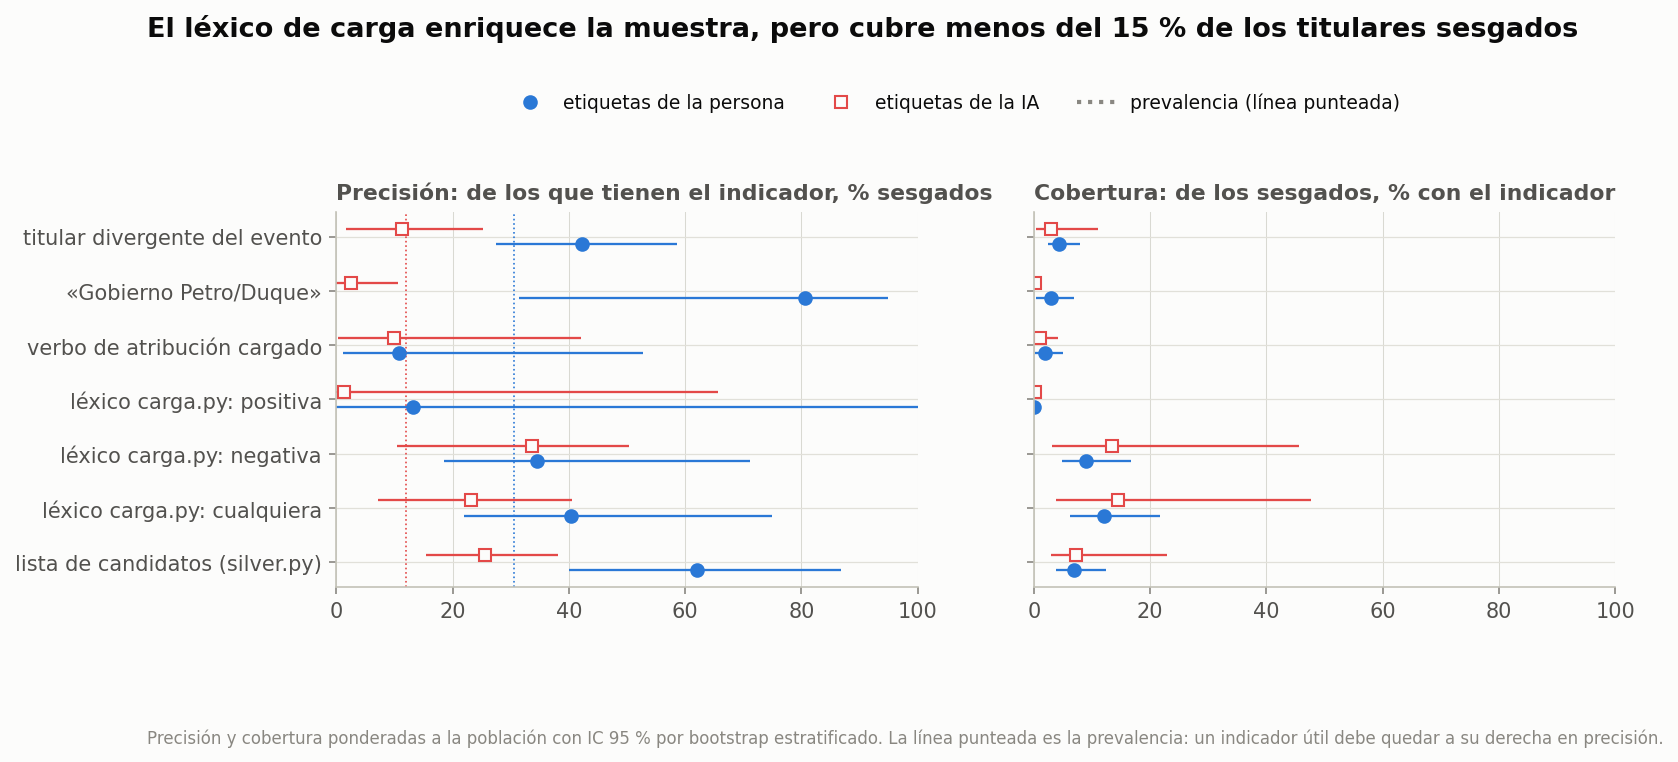
\includegraphics[width=.8\textwidth]{silver/analisis/figuras/38_silver_validacion_indicadores.png}
\caption{Precisión y cobertura (recall) de los indicadores automáticos frente a las
etiquetas, ponderadas a la población, IC 95\,\%.}\label{fig:valid}
\end{figure*}

\subsection{Ejemplos de salida}
La Tabla~\ref{tab:ejemplos} muestra salidas de cada componente. En los titulares
se restituyeron las tildes para facilitar la lectura.

\begin{table*}[t]
\centering\footnotesize
\caption{Ejemplos de salida del modelo. BERTopic: palabras c-TF-IDF y el titular
más cercano al centroide del tópico (coseno). Eventos: titulares de distintos
medios agrupados como el mismo hecho. Silver standard: marca del léxico de carga
frente a las dos etiquetas.}
\label{tab:ejemplos}
\begin{tabularx}{\textwidth}{>{\bfseries}p{2.6cm} p{4.6cm} Y}
\toprule
\textnormal{\textbf{Componente}} & \textbf{Entrada / rasgos} & \textbf{Salida}\\
\midrule
T5 Venezuela, Cuba y Maduro & venezuela, maduro, cuba, venezolanos, nicolas\_maduro, machado & «Venezuela autorizó a Latam para operar entre Bogotá y Caracas» (RCN, 0,94)\\
T4 Policía y delitos & policia, bogota, homicidios, estacion\_policia, cali, hurto & «Atentado de las disidencias de las FARC contra la Policía en Huila» (El Tiempo, 0,91)\\
T17 Reforma a la salud & reforma\_salud, eps, ministro\_salud, sistema\_salud & «Claves de la reforma a la salud presentada por el Gobierno Petro» (Blu Radio, 0,93)\\
\midrule
Evento, 2020-02-07 & 4 medios & «Fernando Ruiz, \textbf{cercano a Vargas Lleras}, es el nuevo ministro de Salud» frente a «Fernando Ruiz Gómez es el nuevo ministro de Salud»\\
Evento, 2025-03-05 & 4 medios; mensaje de urgencia de la reforma a la salud & «\textbf{Gobierno Petro} radicó…» (Blu Radio), «…\textbf{Gobierno Petro insiste}…» (El Tiempo), «\textbf{Armando Benedetti} radicó…» (Caracol), «\textbf{Gobierno} radicó…» (RCN)\\
\midrule
Silver standard & «Gustavo Petro arremete contra Bukele y tacha de falso positivo cifra de homicidios en El Salvador» — léxico: \emph{arremete} & Persona: sesgado (sensacionalismo); IA: sesgado (lenguaje cargado). Acuerdo en sesgo, no en tipo\\
Silver standard & «Polémica por fallo de la Corte Suprema sobre protestas» — léxico: \emph{polémica} & Persona: sesgado (lenguaje cargado); IA: no sesgado. Umbral distinto\\
Silver standard & «Personería suspendió a funcionaria de la UAESP tras escándalo de corrupción» — léxico: \emph{escándalo} & Ninguno lo juzga sesgado: falso positivo del léxico\\
Silver standard & «Venezuela echa por tierra el mito de la no intervención» — sin marca del léxico & Los dos lo juzgan sesgado: falso negativo del léxico\\
\bottomrule
\end{tabularx}
\end{table*}

% ════════════════════════════════════════════════════════════════════════════
\section{ANÁLISIS DE RESULTADOS}
\subsection{Agenda}
El control por sección se lleva la mayoría de los cambios. En el LDA del corpus
completo, de 13 Δ fiables quedan 5 tras el control. Por ejemplo, Fútbol en RCN
pasa de +11,5 a +5,5\pp{} y deja de ser significativo. Con BERTopic y control por
sección sobreviven los cambios de la Tabla~\ref{tab:delta}
(Fig.~\ref{fig:delta}). Con Petro hay más asuntos públicos en cuatro de los cinco
medios; por ejemplo, El Tiempo pasa de 15,8 a 21,8\,\% y Blu Radio de 19,7 a
24,4\,\%. Las agendas también se separan un poco: la distancia Jensen-Shannon
media entre medios pasa de 0,180 a 0,204. Tres hallazgos se repiten en al menos
dos modelos: El Tiempo cubre más inseguridad urbana (+1,1 a +1,7\pp{}) y menos
justicia (−0,7 a −1,1\pp{}), y La República cubre más guerras y geopolítica
(+1,2 a +1,6\pp{}).

\begin{table}[t]
\centering\footnotesize
\caption{Δ relativo significativo con BERTopic y control por sección. Duque y
Petro: participación del tópico en el medio (\%); Δ relativo en pp. Se omiten el tópico mixto 8,
que no es un tema, y Vacunación (+0,4\pp).}
\label{tab:delta}
\setlength{\tabcolsep}{2pt}
\begin{tabular}{llrrl}\toprule
Medio & Tópico & Duque & Petro & Δ rel. (IC 95\,\%)\\\midrule
Caracol & Venezuela y Maduro & 6,6 & 10,0 & +3,8 (2,1; 5,6)\\
Caracol & Policía y delitos & 17,1 & 10,5 & −2,8 (−4,4; −1,2)\\
El Tiempo & Policía y delitos & 7,7 & 7,2 & +1,7 (1,0; 2,4)\\
El Tiempo & Conflicto y víctimas & 12,8 & 9,3 & −1,6 (−2,5; −0,7)\\
La Rep. & Guerras & 1,8 & 3,7 & +1,6 (1,0; 2,2)\\
Caracol & Narcotráfico & 2,7 & 1,7 & −0,9 (−1,3; −0,5)\\
El Tiempo & Narcotráfico & 2,6 & 2,9 & +0,5 (0,3; 0,8)\\
\bottomrule\end{tabular}
\end{table}

\begin{figure*}[t]\centering
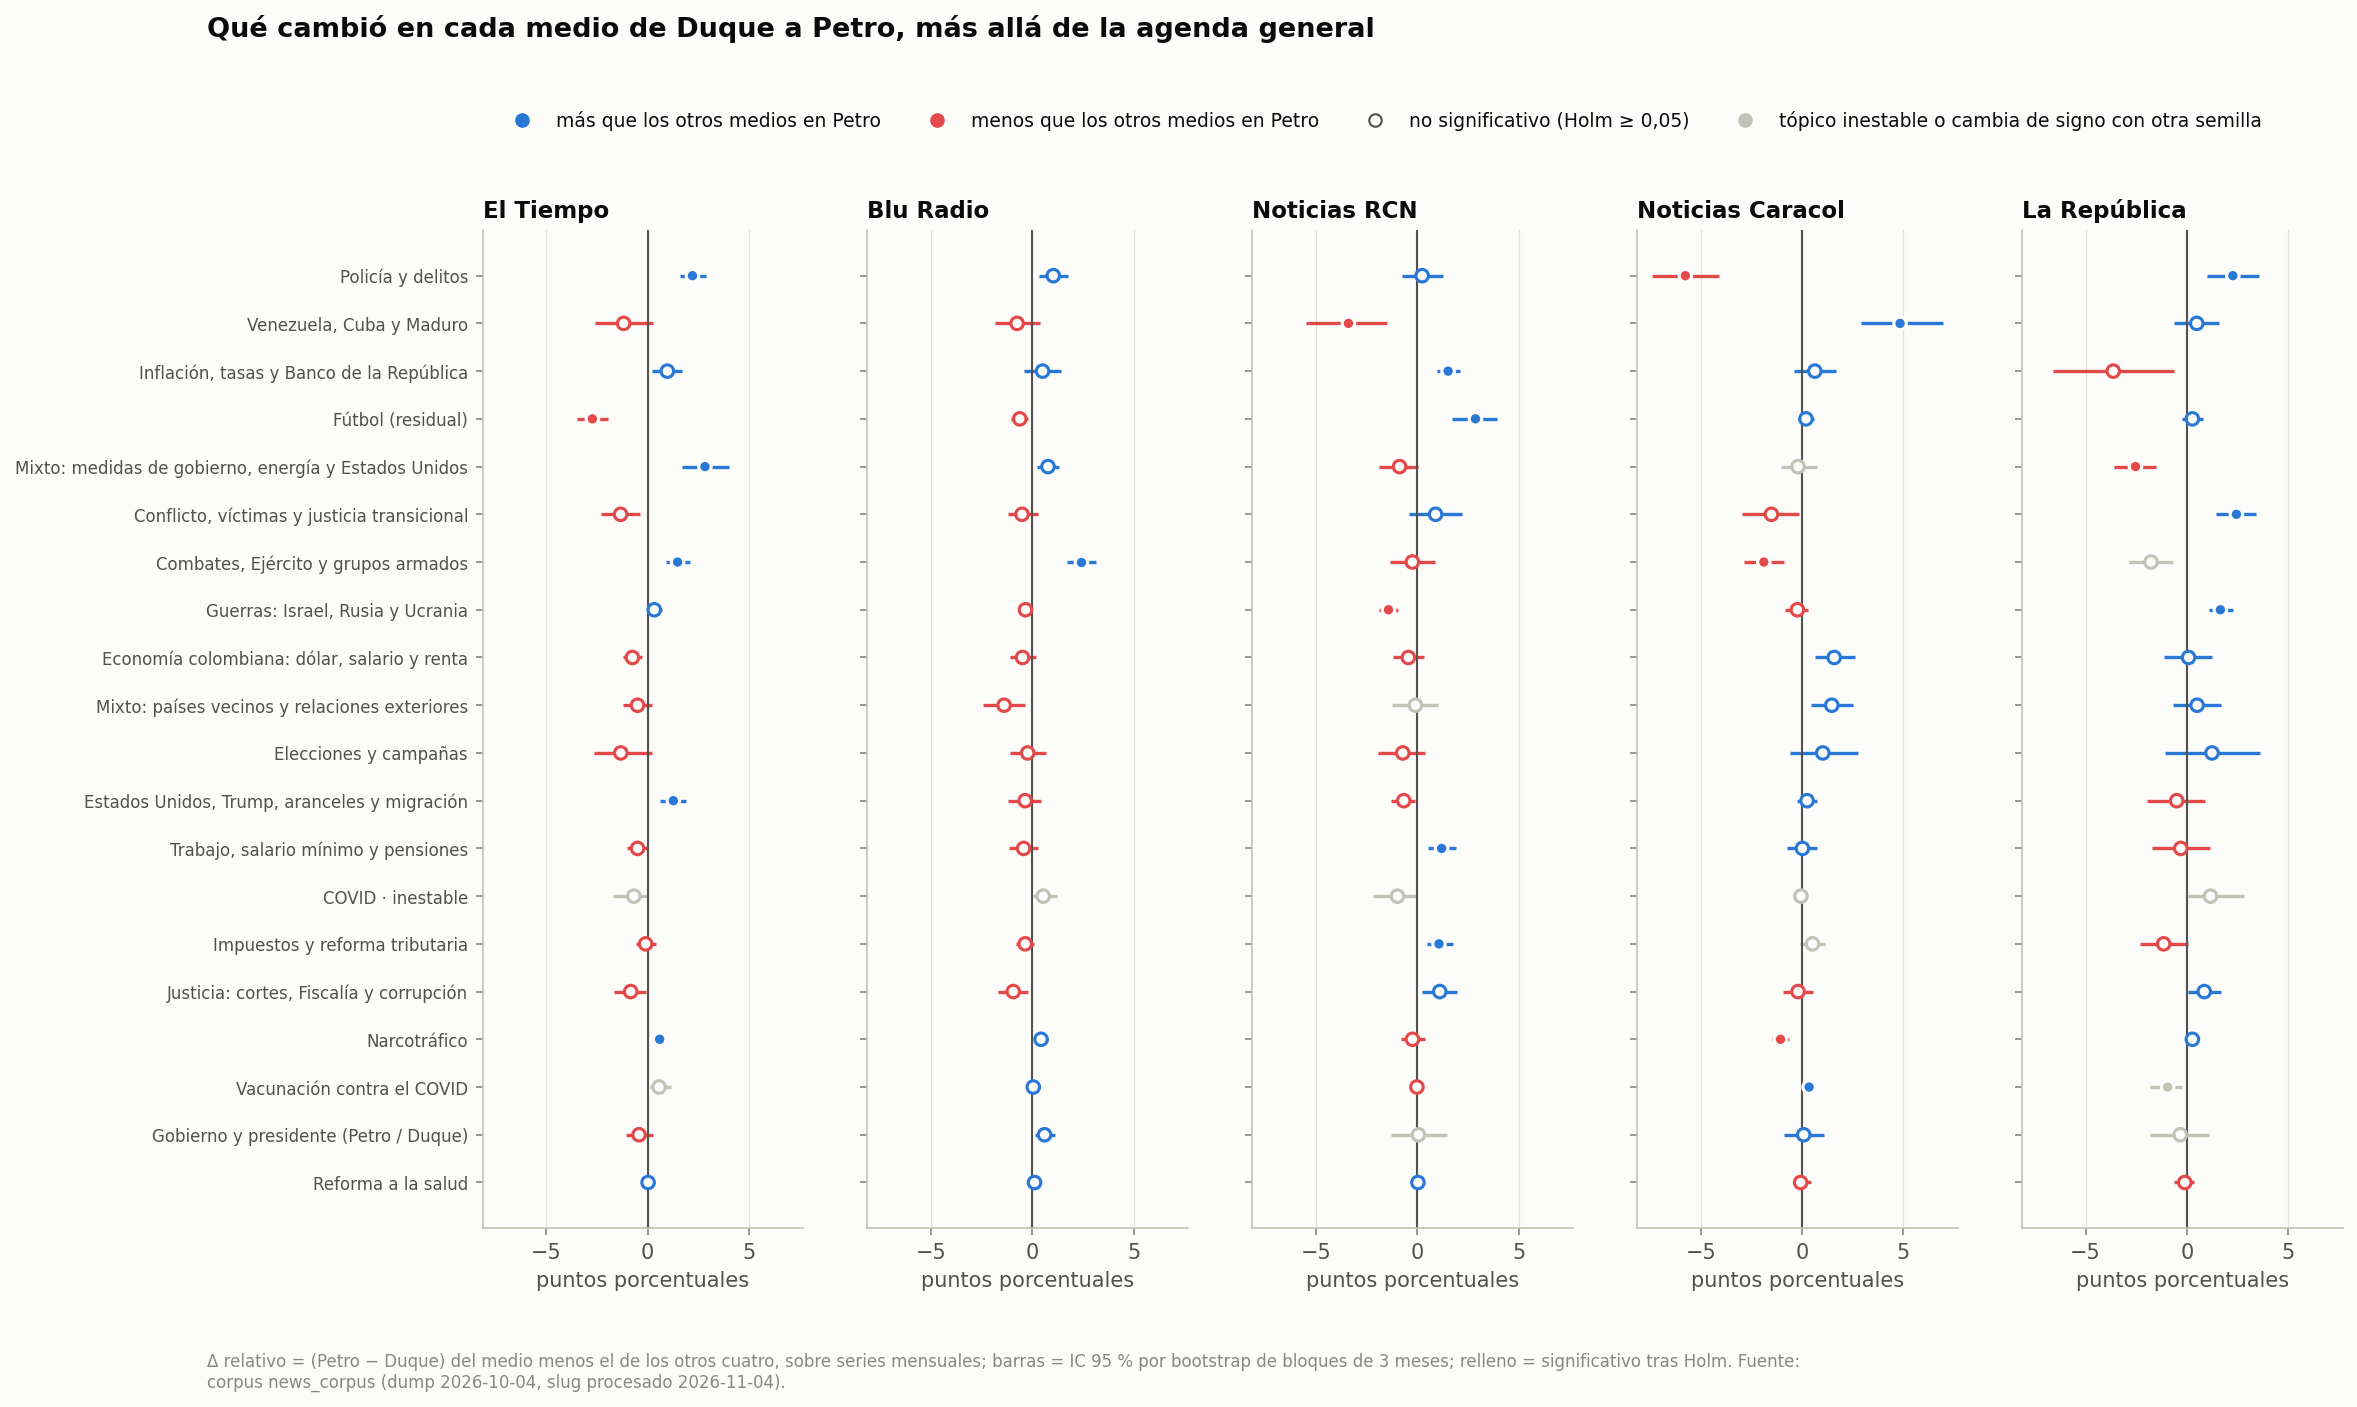
\includegraphics[width=.9\textwidth]{bertopic/figuras/12_delta_relativo.png}
\caption{Δ relativo por medio y tópico (BERTopic, asuntos públicos, con IC 95\,\%).}\label{fig:delta}
\end{figure*}

El Δ relativo puede tener otro signo que el cambio absoluto. Por ejemplo, Policía
y delitos baja en El Tiempo (7,7 → 7,2\,\%), pero baja mucho más en los otros
medios.

\subsection{Selección}
Los perfiles de cada medio son estables entre gobiernos. El más marcado es el de
La República, con $\sim$20\pp{} menos en policía, justicia y conflicto y más en
economía e impuestos: es el perfil de un diario económico, no una omisión. Casi
nada cambia de un gobierno al otro. El único cambio robusto es RCN en Justicia:
+7,5\pp{} frente a los otros medios (IC 2,9--12,7; Fig.~\ref{fig:omision}).
Caracol en Venezuela (+14,4\pp) sólo conserva el signo en las pruebas de
robustez. Como el recall del emparejamiento no está medido, la omisión es una
cota superior.

\begin{figure*}[t]\centering
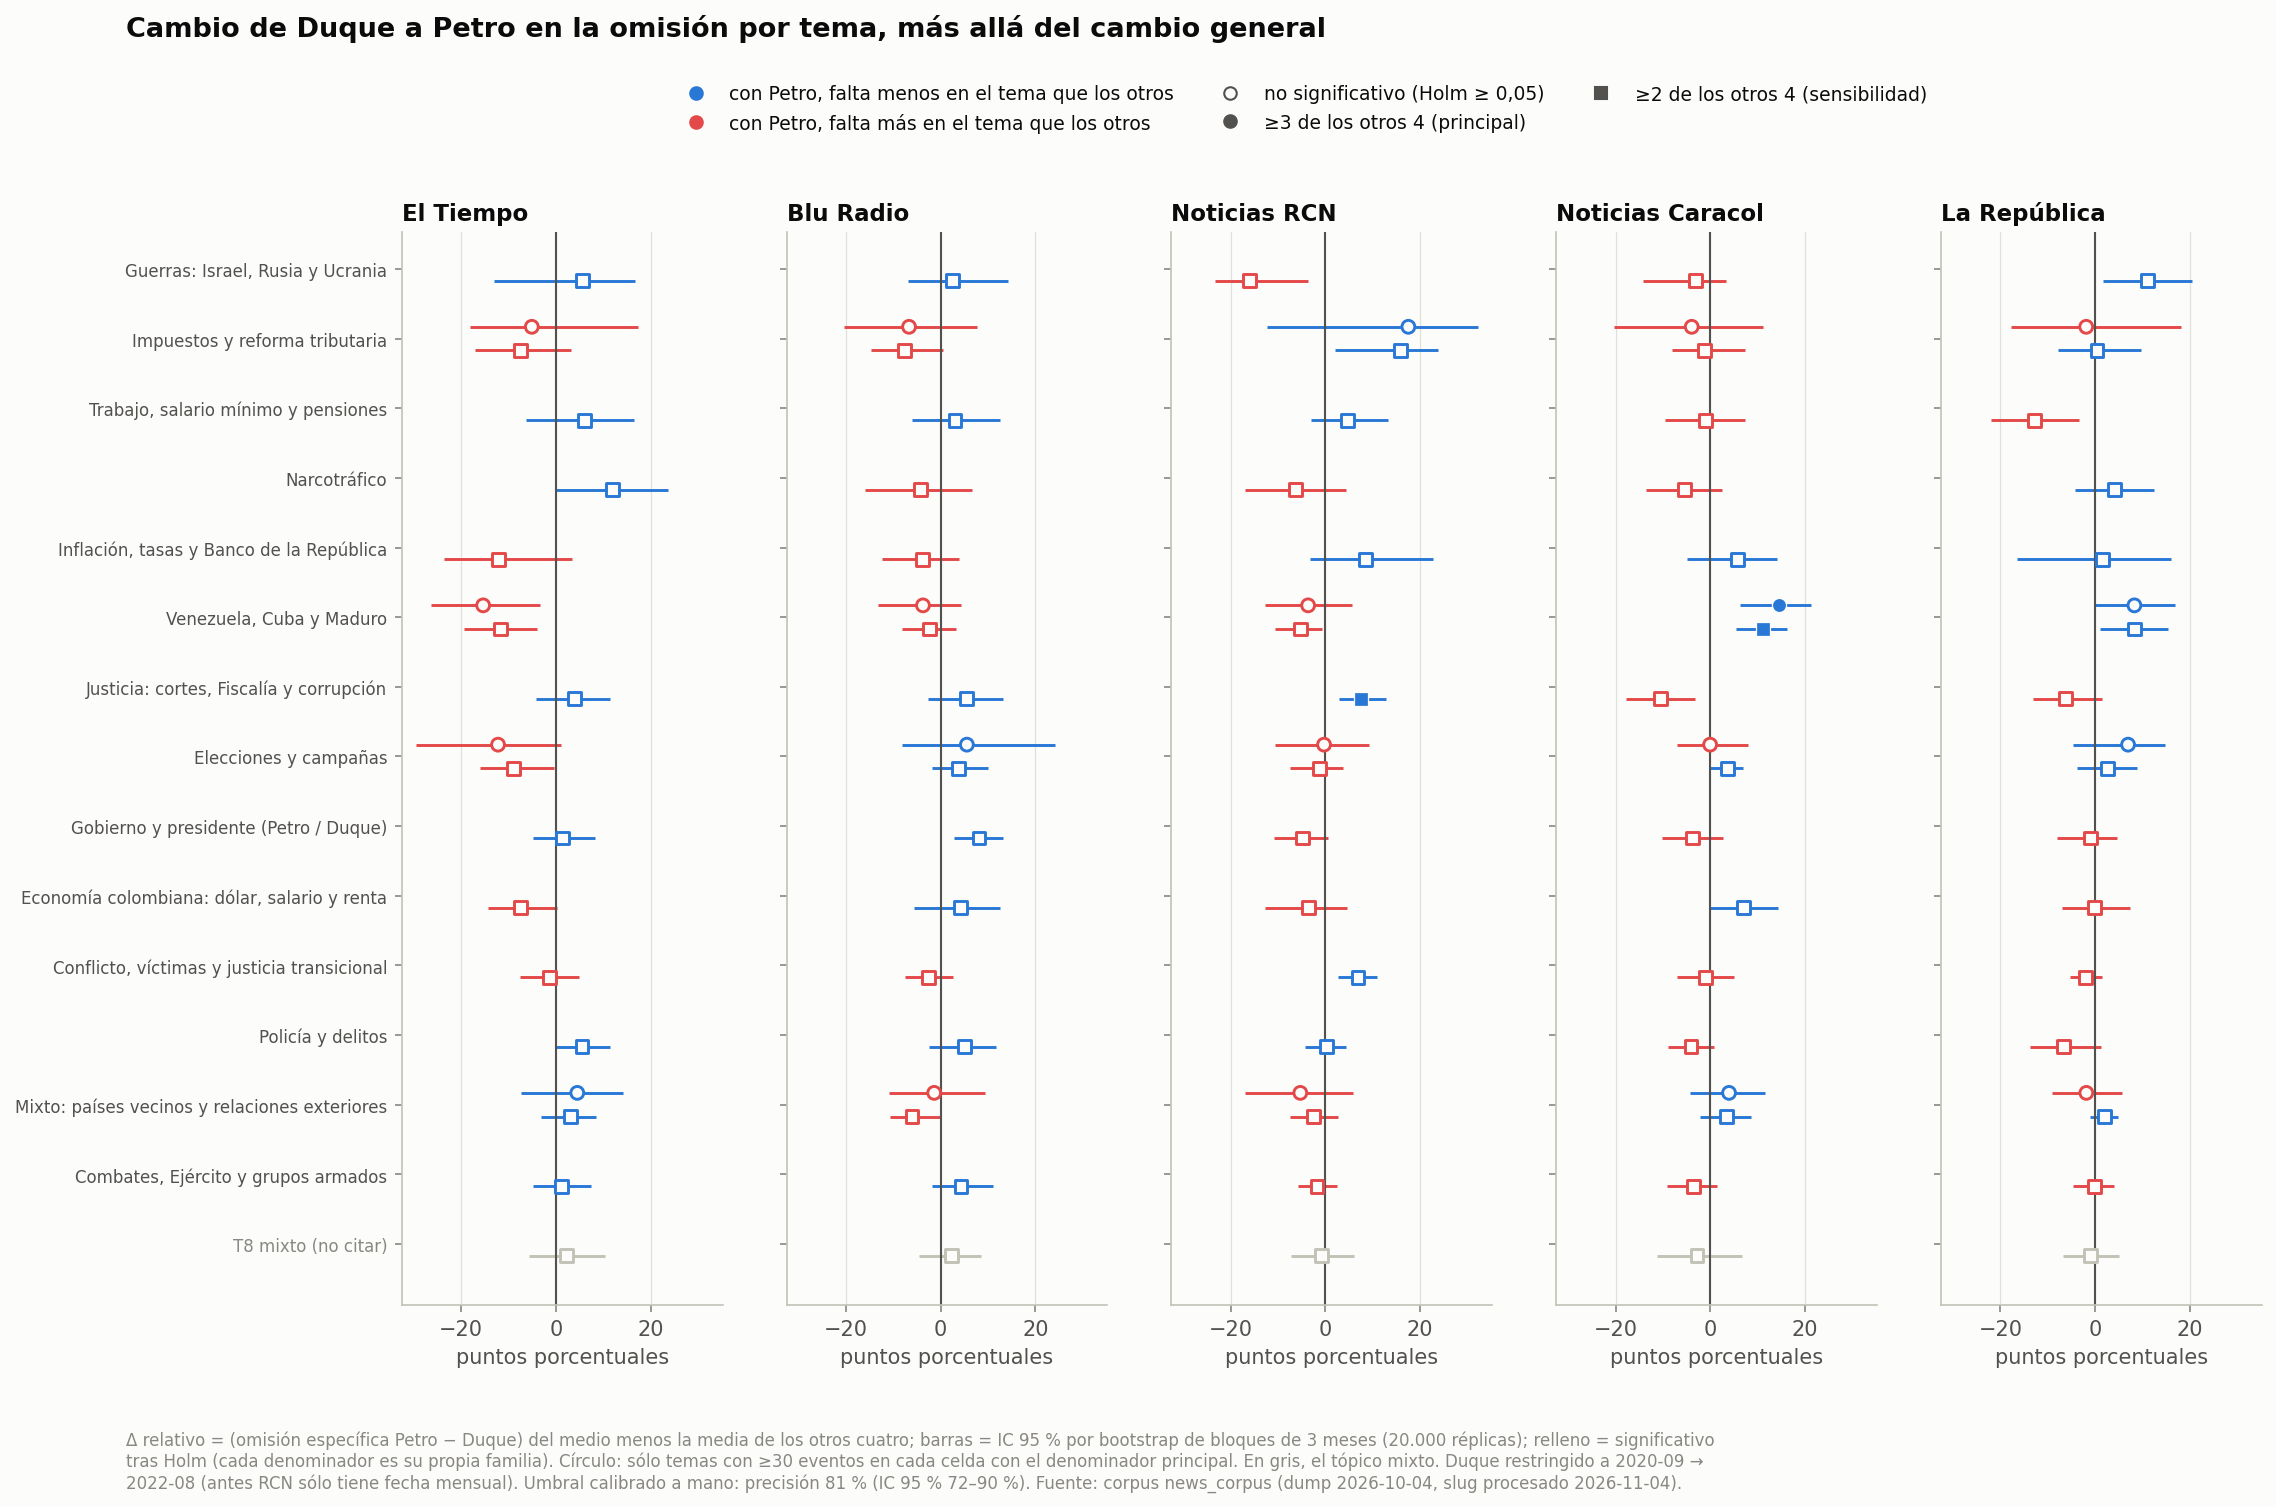
\includegraphics[width=.82\textwidth]{omision/figuras/24_omision_delta_relativo.png}
\caption{Cambio de Duque a Petro en la omisión por tema (Δ relativo frente a los
otros medios, IC 95\,\%).}\label{fig:omision}
\end{figure*}

\subsection{Encuadre}
Las palabras distintivas de cada medio son sobre todo de estilo de casa: El
Tiempo usa nombres completos («Donald Trump» en el 75\,\% de sus titulares sobre
Trump) y Blu Radio formas cortas. El hallazgo más claro es de periodo:
\textbf{todos los medios personalizan más al gobierno con Petro}
(Fig.~\ref{fig:personal}). El Tiempo pasa de 5,1 a 26,9\,\%, Caracol de 7,6 a
28,4\,\%, Blu Radio de 5,4 a 17,0\,\% y RCN de 3,9 a 12,1\,\%; en La República el
cambio no es significativo. Hay 191 eventos de Petro en los que un medio escribe
«Gobierno Petro» y otro sólo «Gobierno», frente a 9 de Duque. Ante los mismos
hechos con Petro, El Tiempo personaliza +11,2\pp{} más que los otros medios, y
RCN (−12,7), La República (−7,9) y Blu Radio (−5,1) menos. Con Duque ningún medio
se distingue.

En carga, las diferencias entre medios ante el mismo hecho son de 3\pp{} como
mucho. Caracol usa más carga negativa con Duque (+2,4\pp) y La República menos
con Petro (−3,1\pp). Blu Radio usa unos +12\pp{} más de verbos de atribución
cargados, en los dos gobiernos. En los titulares sobre el gobierno ningún medio
carga más que los otros, y la carga negativa sube en conjunto de 5,2\,\% a
9,7\,\% con Petro (Fig.~\ref{fig:carga}). En la banda 0,65--0,80 no aparece
encuadre nuevo, y la personalización se mantiene (El Tiempo +15,2\pp).

\begin{figure*}[t]\centering
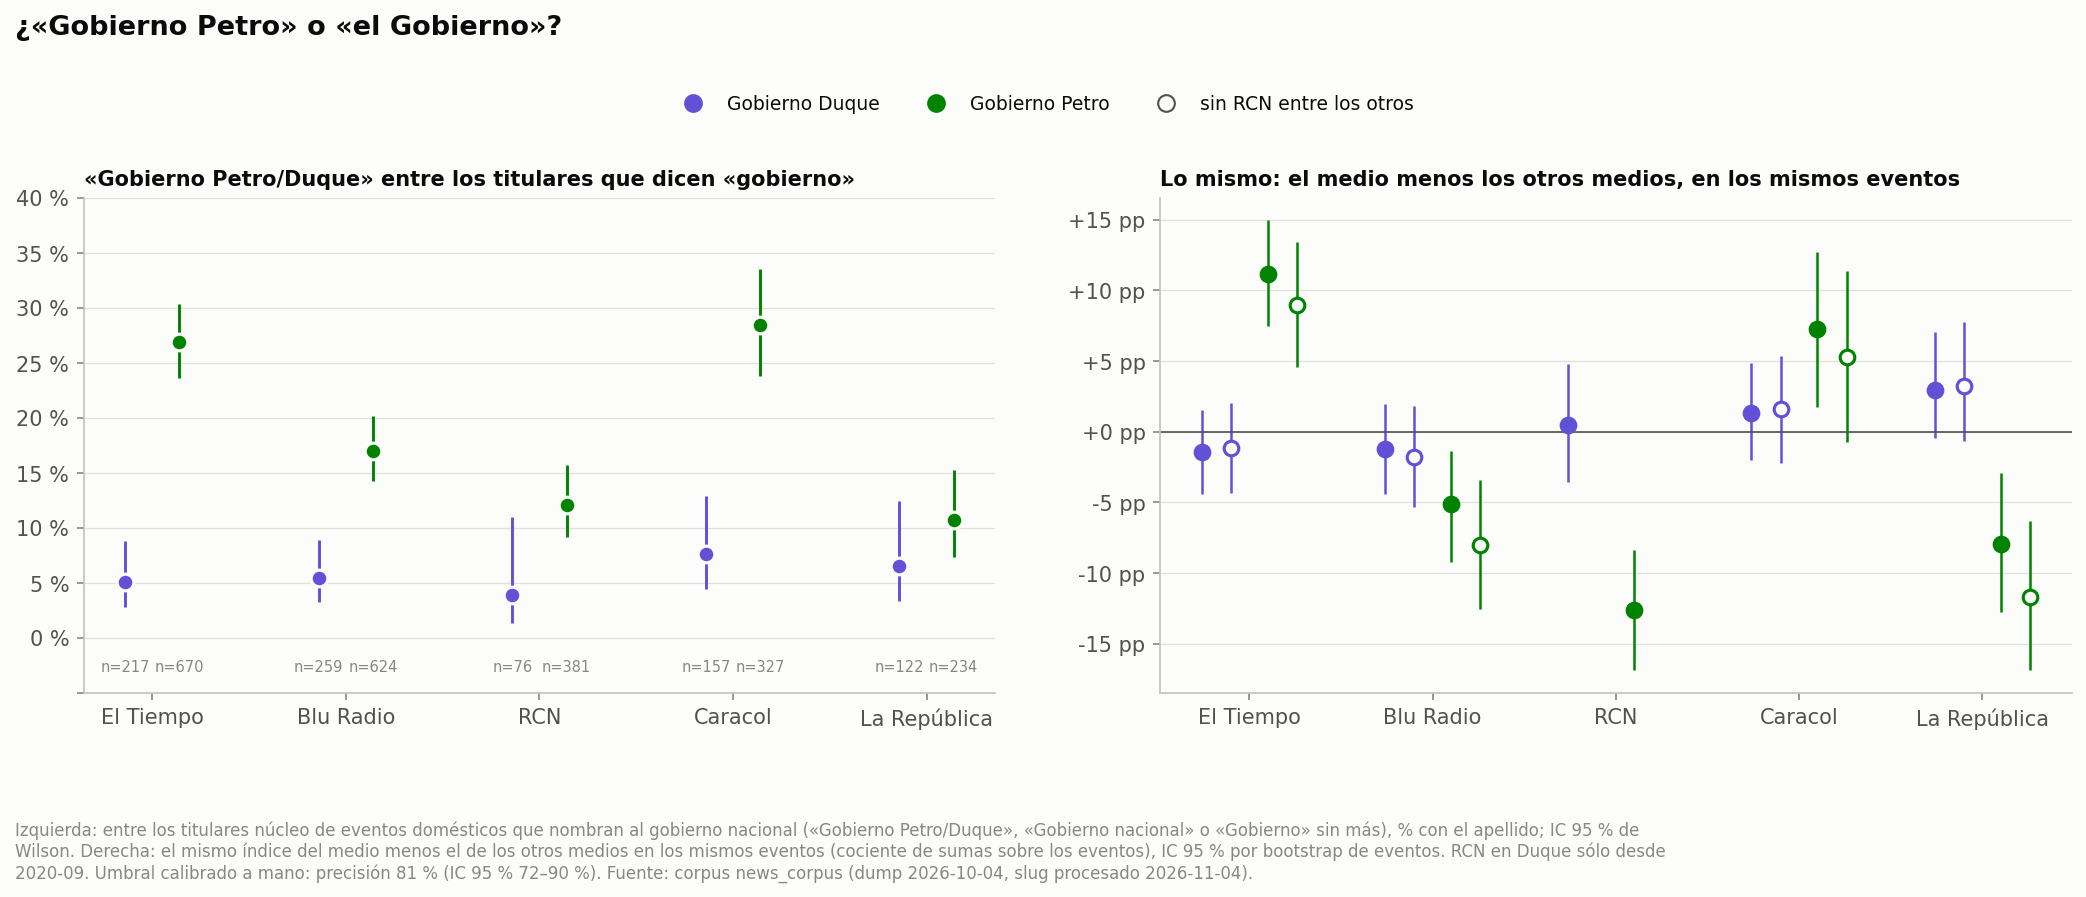
\includegraphics[width=.85\textwidth]{lexico/figuras/29_personalizacion_gobierno.png}
\caption{«Gobierno Petro/Duque» entre los titulares que dicen «gobierno», por
medio y gobierno (izquierda), y frente a los otros medios en los mismos eventos
(derecha).}\label{fig:personal}
\vspace{.6em}
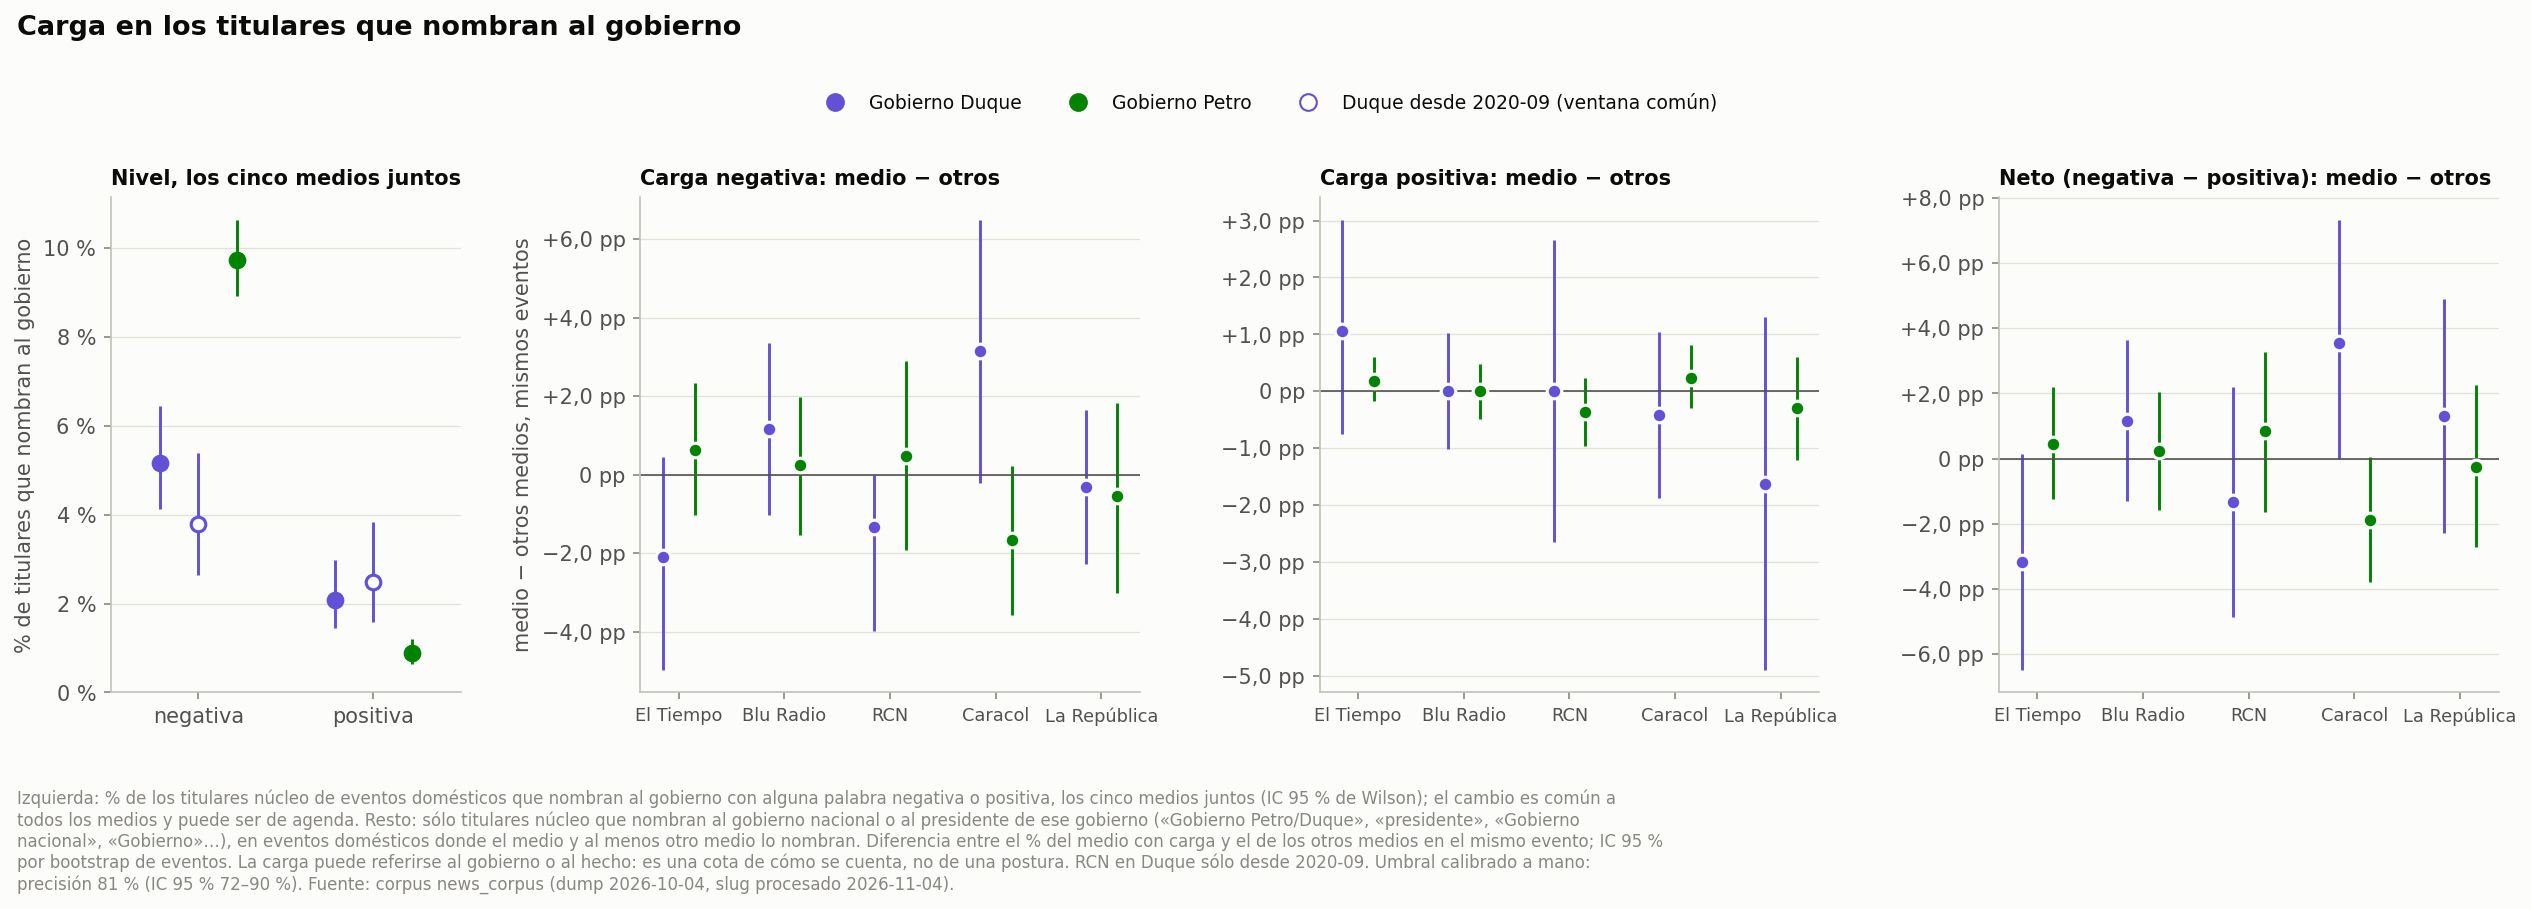
\includegraphics[width=.92\textwidth]{carga/figuras/31_carga_dirigida_gobierno.png}
\caption{Carga en los titulares que mencionan al gobierno: nivel en los cinco
medios y diferencia de cada medio frente a los otros en los mismos eventos.}\label{fig:carga}
\end{figure*}

\subsection{Silver standard}\label{sec:silver}
\begin{figure*}[t]\centering
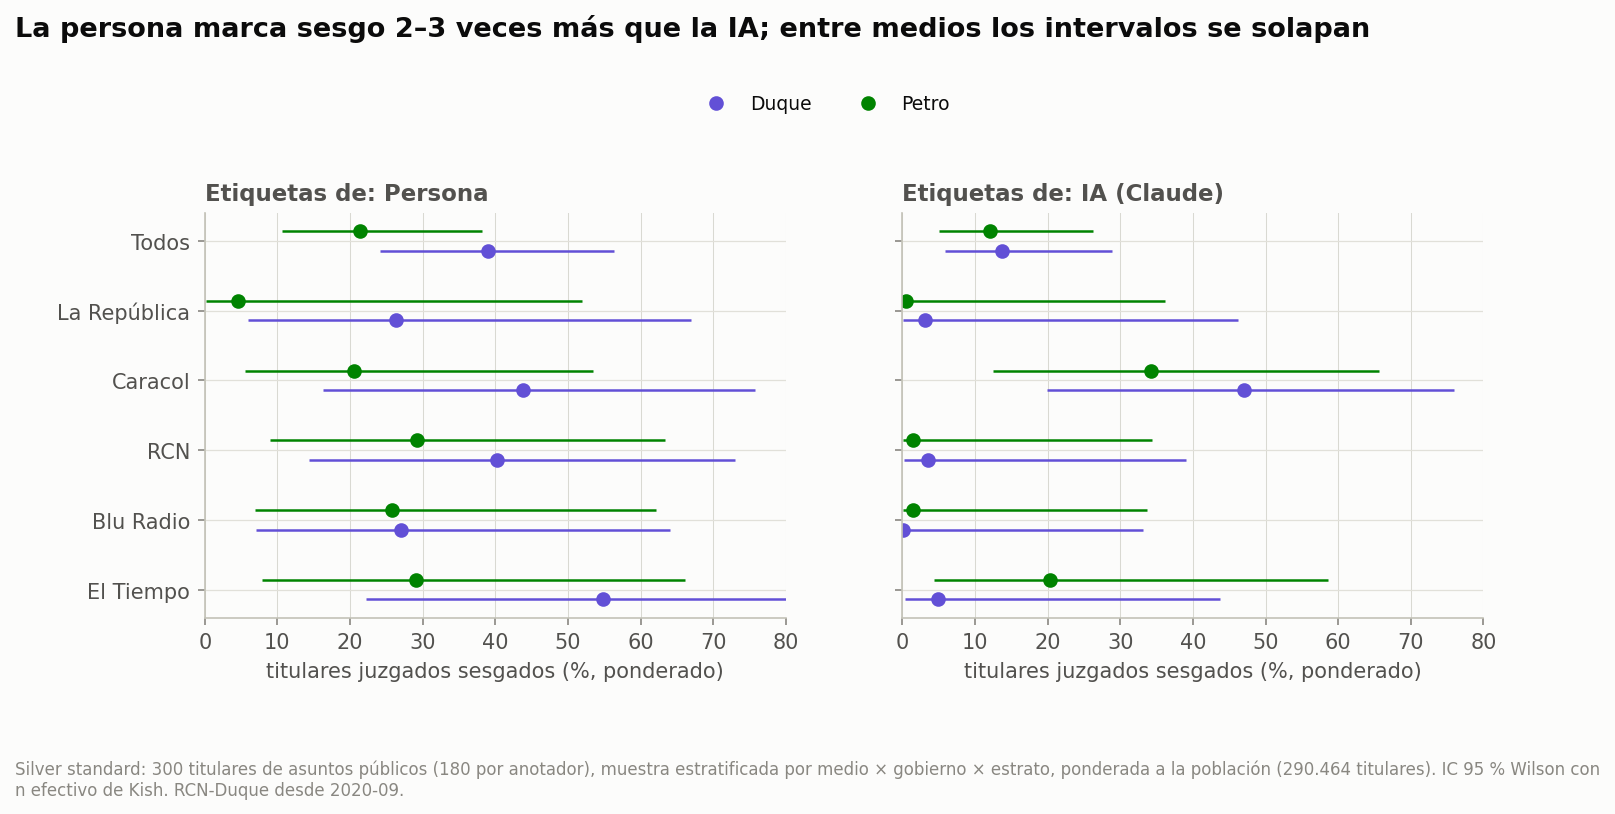
\includegraphics[width=.72\textwidth]{silver/analisis/figuras/36_silver_tasa_sesgo.png}
\caption{Tasa de titulares juzgados sesgados por medio y gobierno, según cada
anotador, ponderada a la población, IC 95\,\%.}\label{fig:silver}
\end{figure*}
El acuerdo entre la persona y la IA es bajo, pero tiene una estructura clara:
κ = 0,30 en «sesgado sí/no» y ≈ 0 en tipo y dirección. En los 60 dobles, la
persona marcó 32 titulares sesgados y la IA 10, y los 10 de la IA están entre los
32 de la persona. Es un umbral distinto, no ruido: la IA aplica la guía al pie de
la letra y no cuenta como sesgo una opinión atribuida a su fuente.

Las tasas ponderadas son de 39\,\% con Duque y 21\,\% con Petro según la persona,
y de 14\,\% y 12\,\% según la IA. \textbf{El sesgo juzgado no sube con Petro},
aunque la carga sí sube. Ninguna diferencia Petro − Duque por medio es
significativa (Fig.~\ref{fig:silver}): con unos 18 titulares por celda y
anotador, los IC son de ±30--50\pp. Según la IA, Caracol es el medio con más
titulares sesgados (41\,\%, IC 21--64). En La República hay un indicio de menos
sesgo desfavorable al gobierno con Petro ($-25$\pp, $p = 0{,}05$ sin corrección
múltiple). La validación de los indicadores automáticos está en
§\ref{sec:clasif}.

\subsection{¿Coinciden los análisis?}
\begin{center}\small\begin{tabular}{L{3.2cm}L{4.4cm}}\toprule
Análisis previo & Silver standard\\\midrule
Carga negativa sube con Petro & El sesgo juzgado no sube: carga ≠ sesgo\\
Personalización sube & Casi nunca se juzga sesgo: es estilo o periodo\\
Blu Radio: verbos cargados & Precisión $\sim$10\,\%: estilo de casa\\
Caracol: más carga con Duque & Tasa más alta según la IA: consistente, débil\\
La República: menos carga con Petro & Menos sesgo desfavorable: indicio\\
\bottomrule\end{tabular}\end{center}

% ════════════════════════════════════════════════════════════════════════════
\section{DISCUSIÓN}
\subsection{Patrones e implicaciones}
\textbf{1. Lo común pesa más que lo propio.} Los cambios más grandes entre Duque
y Petro aparecen en los cinco medios a la vez: más asuntos públicos, más
«Gobierno Petro» y más carga negativa sobre el gobierno. Si cada medio se
comparara sólo consigo mismo, estos cambios se leerían como decisiones
editoriales de cada uno. El Δ relativo y el diseño emparejado por evento son lo
que permite separar el cambio del periodo del cambio de un medio. Que el
gobierno de Petro se nombre como «Gobierno Petro» en todos los medios encaja
mejor con un cambio de periodo, en el estilo del gobierno o en su agenda, que con
una postura de un medio. Este análisis, sin embargo, no puede probar la causa.

\textbf{2. El archivo imita decisiones editoriales.} El control por sección quita
8 de los 13 cambios del LDA, entre ellos el más llamativo, Fútbol en RCN. Eran
cambios en cuánto pesa cada sección en el sitemap, no en qué cubre el medio. La
implicación vale para cualquier estudio sobre archivos web: antes de hablar de
agenda hay que controlar la composición del archivo.

\textbf{3. Carga no es sesgo.} Las palabras cargadas aumentan con Petro y el sesgo
juzgado no. El léxico tiene F1 ≤ 0,22 y no ve el 85\,\% de los titulares
sesgados. Un monitor de sesgo basado en léxicos, o en sentimiento, mediría otra
cosa: sirve para elegir candidatos a revisión (los concentra 1,3--1,9 veces),
no para estimar tasas. Es la advertencia de \cite{grimmer2013}: un método de
diccionario debe validarse sobre el corpus antes de interpretarse.

\textbf{4. El juicio de sesgo depende de quién anota.} Con κ = 0,30, la frontera
entre sesgo y no sesgo a nivel de titular depende del umbral de quien anota. El
modelo de lenguaje aplicó la guía de forma más literal y conservadora: sus «Sí»
son un subconjunto de los de la persona. Sirve como segundo anotador o como
filtro, pero no reemplaza el juicio humano. Cualquier tasa de sesgo de un medio
debería reportarse junto con quién anotó y con qué guía.

\textbf{5. Textos cortos: embeddings antes que LDA.} Con titulares de $\sim$6
palabras útiles, el LDA no da tópicos reproducibles ni con consenso, mientras que
BERTopic repite 19 de 20. Para titulares en español, la estabilidad entre
semillas discrimina mejor entre modelos que la coherencia c\_v.

\subsection{Limitaciones}
\begin{itemize}
\item El segundo anotador del silver standard es un modelo de lenguaje: el κ mide
el acuerdo entre la persona y el modelo, y quedan 32 desacuerdos sin adjudicar.
\item Hay $\sim$18 titulares por medio × gobierno y anotador, con un n efectivo
de $\sim$10, así que los IC por medio son muy anchos.
\item El tipo y la dirección del sesgo no son fiables (κ ≈ 0).
\item Los titulares se reconstruyen desde la URL: no tienen tildes, cifras,
comillas ni signos, y por eso se pierde la atribución de las citas.
\item El emparejamiento acierta en $\sim$81\,\% de los casos y su recall no está
medido.
\item En BERTopic, k = 20 no se eligió con una grilla propia. Cada titular recibe
un solo tópico, y dos tópicos (2 y 8) son mezclas que no deben citarse como tema.
\item RCN tiene fecha exacta sólo desde 2020-09, y el volumen de cada medio
depende de sus sitemaps.
\end{itemize}

\subsection{Mejoras futuras}
\begin{enumerate}
\item Que una segunda persona anote la planilla 2 o adjudique los 32
desacuerdos, para tener un κ entre humanos.
\item Un silver standard centrado en los titulares sobre el gobierno, con
$\sim$100 por celda, para bajar los IC por medio a ±10--15\pp.
\item Medir el recall del emparejamiento anotando ausencias, y calibrar el umbral
del seguimiento.
\item Una grilla de k para BERTopic, extenderlo al corpus completo y validar sus
tópicos con una prueba de intrusión de palabras.
\item Usar el titular publicado o el texto completo en una submuestra, para
recuperar las comillas y la atribución.
\end{enumerate}

% ════════════════════════════════════════════════════════════════════════════
\section{CONCLUSIONES}
Con 1,57 millones de titulares y tres niveles de análisis, las diferencias entre
los cinco medios son pequeñas y sobre todo de perfil y estilo, y esos perfiles se
mantienen entre gobiernos. Lo que cambia con Petro es común a todos: más asuntos
públicos, más personalización y más carga negativa sobre el gobierno. Eso apunta
a un cambio del periodo más que a decisiones editoriales de un medio. Los cambios
propios de cada medio son pocos y modestos: Caracol cubre más Venezuela y menos
policía, RCN más justicia, y El Tiempo personaliza más. Ninguno equivale a un
trato sistemáticamente más duro con un gobierno.

En lo metodológico, BERTopic es el único modelo de tópicos estable sobre
titulares, y el umbral calibrado a mano permite comparar el mismo hecho con una
precisión conocida. El silver standard deja una lección: la carga léxica no
equivale a sesgo juzgado. Cualquier afirmación sobre el sesgo de un medio a
partir de indicadores automáticos de titulares debe tomarse con cautela.

\section*{Reproducibilidad}
El código, los datos procesados y los scripts están en \texttt{entrega3/}.
Hay imágenes Docker (\texttt{duque-petro-lda} y \texttt{duque-petro-bertopic}) y
etapas reproducibles con \texttt{./run.sh}. Se usan las semillas 42, 7 y 123, y
\texttt{config.json} guarda el SHA-256 del input. El código tiene 100 funciones
de prueba. El detalle de cada paso está en \texttt{entrega3/README.md} y en
\texttt{entrega3/INFORME\_FINAL.md}.

{\small
\begin{thebibliography}{99}
\setlength{\itemsep}{1pt}
\bibitem{entman} R. Entman. Framing: Toward Clarification of a Fractured Paradigm. \emph{Journal of Communication}, 43(4), 51--58, 1993.
\bibitem{hamborg2019} F. Hamborg, K. Donnay y B. Gipp. Automated identification of media bias in news articles: an interdisciplinary literature review. \emph{International Journal on Digital Libraries}, 20, 391--415, 2019.
\bibitem{hamborg2020} F. Hamborg. Media Bias, the Social Sciences, and NLP: Automating Frame Analyses to Identify Bias by Word Choice and Labeling. \emph{ACL Student Research Workshop}, 2020.
\bibitem{lda} D. Blei, A. Ng y M. Jordan. Latent Dirichlet Allocation. \emph{Journal of Machine Learning Research}, 3, 993--1022, 2003.
\bibitem{roder2015} M. Röder, A. Both y A. Hinneburg. Exploring the Space of Topic Coherence Measures. \emph{WSDM}, 399--408, 2015.
\bibitem{bertopic} M. Grootendorst. BERTopic: Neural topic modeling with a class-based TF-IDF procedure. arXiv:2203.05794, 2022.
\bibitem{reimers2019} N. Reimers e I. Gurevych. Sentence-BERT: Sentence Embeddings using Siamese BERT-Networks. \emph{EMNLP-IJCNLP}, 2019.
\bibitem{reimers2020} N. Reimers e I. Gurevych. Making Monolingual Sentence Embeddings Multilingual using Knowledge Distillation. \emph{EMNLP}, 2020.
\bibitem{umap} L. McInnes, J. Healy y J. Melville. UMAP: Uniform Manifold Approximation and Projection for Dimension Reduction. arXiv:1802.03426, 2018.
\bibitem{kunsch1989} H. Künsch. The Jackknife and the Bootstrap for General Stationary Observations. \emph{The Annals of Statistics}, 17(3), 1217--1241, 1989.
\bibitem{holm1979} S. Holm. A Simple Sequentially Rejective Multiple Test Procedure. \emph{Scandinavian Journal of Statistics}, 6(2), 65--70, 1979.
\bibitem{cohen1960} J. Cohen. A Coefficient of Agreement for Nominal Scales. \emph{Educational and Psychological Measurement}, 20(1), 37--46, 1960.
\bibitem{monroe2008} B. Monroe, M. Colaresi y K. Quinn. Fightin' Words: Lexical Feature Selection and Evaluation for Identifying the Content of Political Conflict. \emph{Political Analysis}, 16(4), 372--403, 2008.
\bibitem{bh1995} Y. Benjamini e Y. Hochberg. Controlling the False Discovery Rate: A Practical and Powerful Approach to Multiple Testing. \emph{Journal of the Royal Statistical Society B}, 57(1), 289--300, 1995.
\bibitem{wilson1927} E. Wilson. Probable Inference, the Law of Succession, and Statistical Inference. \emph{Journal of the American Statistical Association}, 22(158), 209--212, 1927.
\bibitem{kish} L. Kish. \emph{Survey Sampling}. Wiley, 1965.
\bibitem{grimmer2013} J. Grimmer y B. Stewart. Text as Data: The Promise and Pitfalls of Automatic Content Analysis Methods for Political Texts. \emph{Political Analysis}, 21(3), 267--297, 2013.
\end{thebibliography}
}
\end{document}
